Além do operador de Sobel, existem vários outros operadores baseados em gradiente. Um deles é o Prewitt \autocite{ref:prewitt}, caracterizado por dois \textit{kernels} $3 \times 3$, com apenas $0$, $1$ e $-1$. No caso da \cref{fig:h11}, o gradiente está apontando para a direção $(-1, -1)$, isto é, da direita-inferior para a esquerda-superior.

Na \cref{fig:grad}, podemos ver claramente o direcionamento pelas antenas da borboleta. A antena esquerda, que está alinhada com a borboleta, fica quase indetectada pelo filtro, enquanto a antena direita aparece de forma bem marcada. Além disso, na antena direta, apenas uma das bordas fica marcada, isso porque o filtro não depende apenas da angulação, mas do direcionamento positivo ou negativo naquele ângulo.

O operador de Prewitt, quando usado com direções ortogonais, também pode ser combinado como o de Sobel (\cref{sec:sobel}).

\begin{figure}[H]
    \centering
    \begin{subfigure}{0.48\textwidth}
        \centering
        \begin{kmatrix}
    \matrix[square matrix]{
        -1 & -1 & 0 \\
        -1 & 0 & 1 \\
        0 & 1 & 1 \\
    };
\end{kmatrix}

        \caption{Máscara $h_{11}$.}
        \label{fig:h11}
    \end{subfigure}%
    \begin{subfigure}{0.48\textwidth}
        \centering
        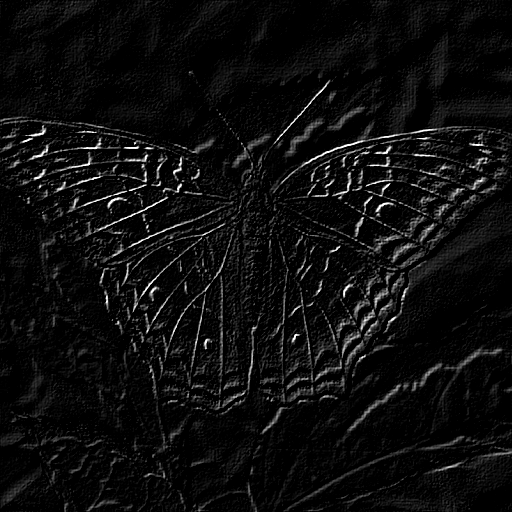
\includegraphics[width=0.9\textwidth]{resultados/butterfly_h11.png}
        \caption{Convolução com $h_{11}$.}
        \label{fig:grad}
    \end{subfigure}

    \caption{Operador de Prewitt, com exemplo.}
\end{figure}

A aplicação do filtro pode ser feita por:

\begin{minted}{bash}
    $ python3 main.py imagens/butterfly h11
\end{minted}
